%! suppress = MissingImport
%! suppress = MissingLabel
%! suppress = LineBreak

% CLI args https://tex.stackexchange.com/a/1501
\newif\ifhandout
\input{flags}

%! suppress = MissingLabel
%! suppress = DocumentclassNotInRoot
%! suppress = DiscouragedUseOfDef

% * Make friends tikz & colors
%   https://en.wikibooks.org/wiki/LaTeX/Colors
% * To enable vertical top alignment globally
%   https://tex.stackexchange.com/questions/9889/positioning-content-at-the-top-of-a-beamer-slide-by-default
% * Set handout from CLI
%   https://tex.stackexchange.com/a/1501
\ifhandout
\documentclass[usenames, dvipsnames, handout]{beamer} % https://tex.stackexchange.com/questions/224091/beamer-how-to-disable-pause-temporarily
\else
\documentclass[usenames, dvipsnames]{beamer}
\fi
% ------------------------------------------------

% Graphics
\usepackage{color}
\usepackage{tabularx}
\usepackage{tikz}
% https://tikz.dev/tikz-graphs
\usetikzlibrary{positioning, shapes.geometric, arrows, automata, graphs}
\tikzset{
    expr/.style={ellipse, draw=gray!60, fill=gray!5, very thick, minimum size=7mm, yshift=0.7cm},
    hexpr/.style={ellipse, draw=gray!60, fill=blue!15, very thick, minimum size=7mm, yshift=0.7cm},
    stmt/.style={rectangle, draw=gray!60, fill=gray!5, very thick, minimum size=5mm, yshift=0.7cm},
    decl/.style={rectangle, draw=blue!60, fill=gray!5, very thick, minimum size=5mm, yshift=0.7cm},
    hdecl/.style={rectangle, draw=blue!60, fill=blue!15, very thick, minimum size=5mm, yshift=0.7cm},
    subtree/.style={shape border rotate=90, isosceles triangle, draw=gray!60, fill=gray!5, very thick, minimum size=5mm, yshift=0.0cm},
}
\usepackage{blkarray}
\usepackage{graphicx}
\usepackage{forest} % https://tex.stackexchange.com/questions/198405/how-to-change-the-color-of-subtrees-in-tikz-qtree
% ------------------------------------------------

% Math
\usepackage{amsmath, amsfonts}
\usepackage{amssymb}
\usepackage{proof}
\usepackage{mathrsfs}
% Crossed-out symbols
% https://tex.stackexchange.com/questions/75525/how-to-write-crossed-out-math-in-latex
\usepackage[makeroom]{cancel}
\usepackage{mathtools}
% ------------------------------------------------

% Additional font sizes
% https://www.overleaf.com/learn/latex/Questions/How_do_I_adjust_the_font_size%3F
\usepackage{moresize}
% Additional colors
% https://www.overleaf.com/learn/latex/Using_colours_in_LaTeX
\usepackage{xcolor}
% Textual math symbols
\usepackage{textcomp}
% ------------------------------------------------

% Language
\usepackage[utf8] {inputenc}
\usepackage[T2A] {fontenc}
\usepackage[english, russian] {babel}
\usepackage{indentfirst, verbatim}
\usetikzlibrary{cd, babel}
% ------------------------------------------------

% Fonts: https://sites.math.washington.edu/~reu/docs/latex_symbols.pdf
\usepackage{stmaryrd}
\usepackage{cmbright}
\usepackage{wasysym}
\usepackage[weather]{ifsym} % https://tex.stackexchange.com/questions/100424/how-to-use-the-ifsym-package
% https://tex.stackexchange.com/questions/615300/pdflatex-builtin-glyph-names-is-empty
\pdfmapline{=dictsym DictSym <dictsym.pfb}
\pdfmapline{=pigpen <pigpen.pfa}
\usepackage{dictsym}
% ------------------------------------------------

% Code
% * Needs -shell-escape build flag
%   https://tex.stackexchange.com/questions/99475/how-to-invoke-latex-with-the-shell-escape-flag-in-texstudio-former-texmakerx
% * Set build directory
%   https://tex.stackexchange.com/questions/339931/latex-minted-package-using-custom-output-directory-build
\usepackage{minted}
\setminted{xleftmargin=\parindent, autogobble, escapeinside=\#\#}
% ------------------------------------------------

% Template
\usetheme{CambridgeUS}
\usecolortheme{dolphin}
% https://tex.stackexchange.com/questions/231439/beamer-how-to-make-font-larger-for-page-numbers
\setbeamerfont{headline}{size=\scriptsize}
\setbeamerfont{footline}{size=\scriptsize}
% Remove heddline
% https://tex.stackexchange.com/questions/33146/how-could-i-remove-a-header-in-a-beamer-presentation
%\setbeamertemplate{headline}{}
% Slide sizes
% https://tex.stackexchange.com/questions/56768/how-to-set-a-small-default-font-size-with-beamer
%\geometry{paperwidth=140mm,paperheight=105mm} % 4:3
\geometry{paperwidth=168mm,paperheight=105mm} % 16:10
% Remove navigation bar
% https://stackoverflow.com/questions/3210205/how-to-get-rid-of-navigation-bars-in-beamer
\beamertemplatenavigationsymbolsempty
% ------------------------------------------------

% Bullets
% https://9to5science.com/change-bullet-style-formatting-in-beamer
% https://tex.stackexchange.com/questions/185742/i-need-to-change-color-of-beamer-itemize-and-subitem-separately
\setbeamertemplate{itemize item}{\scriptsize\raise1.25pt\hbox{\donotcoloroutermaths$\blacktriangleright$}}
\setbeamertemplate{itemize subitem}{\scriptsize\raise1.5pt\hbox{\donotcoloroutermaths$\blacktriangleright$}}
\setbeamertemplate{itemize subsubitem}{\tiny\raise1.5pt\hbox{\donotcoloroutermaths$\blacktriangleright$}}
\setbeamertemplate{enumerate item}{\insertenumlabel.}
\setbeamertemplate{enumerate subitem}{\insertenumlabel.\insertsubenumlabel}
\setbeamertemplate{enumerate subsubitem}{\insertenumlabel.\insertsubenumlabel.\insertsubsubenumlabel}
% ------------------------------------------------

% Table of contents format
% https://tex.stackexchange.com/questions/642927/format-table-of-contents-in-beamer
\setbeamertemplate{section in toc}{%
        {\color{blue}\inserttocsectionnumber.}
    \inserttocsection\par%
}
\setbeamertemplate{subsection in toc}{%
        {\color{blue}\hspace{1em}\scriptsize\raise1.25pt\hbox{\donotcoloroutermaths$\blacktriangleright$}}
    \inserttocsubsection\par%
}
\setbeamertemplate{subsubsection in toc}{%
        {\color{blue}\hspace{2em}\tiny\raise1.25pt\hbox{\donotcoloroutermaths$\blacktriangleright$}}
    \inserttocsubsubsection\par%
}
% ------------------------------------------------

% Misc
\usepackage{multicol}
\usepackage{hyperref}
\usepackage{soul} % https://tex.stackexchange.com/questions/23711/strikethrough-text
% ------------------------------------------------

% Fix \pause for amsmath package envs (black black magic)
% https://tex.stackexchange.com/questions/16186/equation-numbering-problems-in-amsmath-environments-with-pause/75550#75550
% https://tex.stackexchange.com/questions/6348/problem-with-beamers-pause-in-alignments
%! suppress = Makeatletter
\makeatletter
\let\save@measuring@true\measuring@true
\def\measuring@true{%
    \save@measuring@true
    \def\beamer@sortzero##1{\beamer@ifnextcharospec{\beamer@sortzeroread{##1}}{}}%
    \def\beamer@sortzeroread##1<##2>{}%
    \def\beamer@finalnospec{}%
}
%! suppress = Makeatletter
\makeatother
% ------------------------------------------------

% Sections
\newcommand{\sectionplan}[1]{\section{#1}%
    \begin{frame}[noframenumbering]{Содержание}
        \tableofcontents[currentsection]
    \end{frame}
}
\newcommand{\subsectionplan}[1]{\subsection{#1}%
    \begin{frame}[noframenumbering]{Содержание}
        \tableofcontents[currentsubsection]
    \end{frame}
}
% ------------------------------------------------

% Footnotes
\renewcommand{\thefootnote}{\arabic{footnote}}
\renewcommand{\thempfootnote}{\arabic{mpfootnote}}
% https://tex.stackexchange.com/questions/28465/multiple-footnotes-at-one-point
\usepackage{fnpct}
% ------------------------------------------------

% Links
% Colors also links on slide foot.
%\hypersetup{
%    colorlinks=true,
%    citecolor=blue,
%    linkcolor=blue,
%    urlcolor=blue
%}
% ------------------------------------------------

% Appendix
% Slide numbers
% https://tex.stackexchange.com/questions/70448/dont-count-backup-slides
\usepackage{appendixnumberbeamer}
\newcommand{\backupbegin}{
    \newcounter{framenumbervorappendix}
    \setcounter{framenumbervorappendix}{\value{framenumber}}
}
\newcommand{\backupend}{
    \addtocounter{framenumbervorappendix}{-\value{framenumber}}
    \addtocounter{framenumber}{\value{framenumbervorappendix}}
}
% ------------------------------------------------

% Custom commands
% * Decor
\newcommand{\newtopic}[0]{$+$} % item: new topic on "in previous series"
\newcommand{\then}{$\Rightarrow$} % item: consequences
\newcommand{\pop}[0]{\SunCloud} %item:  general eduation
\newcommand{\popslide}[0]{(\pop)}
\newcommand{\advanced}[0]{$\varhexstar$} % item: advanced science
\newcommand{\advancedslide}[0]{(\advanced)}
\newcommand{\practical}[0]{\dstechnical} % item: practical programming notions
\newcommand{\practicalslide}[0]{(\practical)}
\newcommand{\todo}[0]{todo} % item: question
\newcommand{\answer}[0]{\Lightning} % item: answer to the previous question
\newcommand{\eg}[0]{e.g.} % item: example
\newcommand{\defi}[0]{$\Delta$} % item: definition on smth
\newcommand{\textdefi}[1]{\textbf{#1}}
\newcommand{\positive}{$+$} % item: pros
\newcommand{\negative}{{\color{red} $-$}} % item: cons
\newcommand%! suppress = EscapeHashOutsideCommand
\NB[1][0.3]{N\kern-#1em{B}} % default kern amount: -0.3em
\renewcommand{\emph}[1]{{\color{blue} \textit{#1}}}
\newcommand{\vocab}[1]{\textbf{#1}} % item: important new word
% * Lambda calculi
\newcommand{\comb}[1]{\mathbf{#1}} % defined combinator
\newcommand{\term}[1]{\mathbf{#1}} % predefined lambda-term reference
\newcommand{\termdef}{\coloneqq} % lamda term binding
\newcommand{\step}{\rightsquigarrow} % reduction step
\newcommand{\sstep}{\twoheadrightarrow} % multiple steps reduction
\newcommand{\ap}{~} % lambda-term application
\newcommand{\subst}[3]{\left[#2 \mapsto #3 \right] #1} % substitution
\newcommand{\eqbeta}{=_\beta} % beta equality
\newcommand{\eqeta}{=_\eta} % eta-equality
\newcommand{\eqt}{=} % tree-equality of terms
\newcommand{\tlist}[1]{\term{[}#1\term{]}} % list-term
% * Legacy
%\newcommand{\err}[0]{\textcolor{red}{ошибка}} % compilation error

% ------------------------------------------------

% Speaker notes
% https://tex.stackexchange.com/questions/114219/add-notes-to-latex-beamer
% https://tex.stackexchange.com/questions/35444/split-beamer-notes-across-multiple-notes-pages/35496#35496
%\setbeameroption{show notes on second screen=right} % enable speaker notes
%--------------------------------------

\author[]{Андрей Стоян, Илья Колегов, Дмитрий Халанский}
\institute[MSE ITMO]{MSE ITMO}

\setminted{xleftmargin=\parindent, autogobble, escapeinside=??}
\newcommand{\iso}{\sim}

\title{4. Типы данных}
\author{Андрей Стоян}
\institute[ИПКН ИТМО]{ИПКН ИТМО}

\date{осень 2025}

\begin{document}

    \mymaketitle

    \begin{frame}[noframenumbering]{Содержание}
        \tableofcontents
    \end{frame}

    \sectionplan{Вариантность}

    \begin{frame}[fragile]{(Ковариантный) функтор}
        \pause
        \begin{minted}{haskell}
            class Functor f where
              fmap :: (a -> b) -> (f a -> f b)
        \end{minted}
        \vspace{1em}
        \begin{figure}[H]
            \centering
            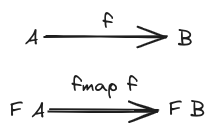
\includegraphics[width=0.3\textwidth]{figs/functor}
        \end{figure}
    \end{frame}

    \begin{frame}[fragile]{Контравариантный функтор}
        \pause
        \begin{minted}{haskell}
            class Contravariant f where
              contramap :: (a -> b) -> (f b -> f a)
        \end{minted}
        \vspace{1em}
        \begin{figure}[H]
            \centering
            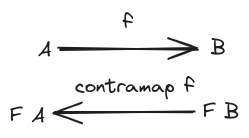
\includegraphics[width=0.3\textwidth]{figs/contra-functor}
        \end{figure}
    \end{frame}

    \begin{frame}[fragile]{Знак позиции}
        \pause
        \begin{center}
            \begin{tabular}[h]{|c|c|c|}
                \hline
                Тип                              & знак позиции \mintinline{haskell}{A} & знак позиции \mintinline{haskell}{B} \\
                \hline
                \mintinline{haskell}{Either A B} & \pause $+$                                  & $+$                                  \\
                \mintinline{haskell}{(A, B)}     & \pause $+$                                  & $+$                                  \\
                \mintinline{haskell}{A -> B}     & \pause $-$                                  & $+$                                  \\
                \hline
            \end{tabular}
        \end{center}
        \vspace{1em}
        \begin{itemize}
            \item[\todo] \pause \mintinline{haskell}{f :: ((A, B) -> C) -> (D, E)}
            \item[\todo] \pause Объявите \mintinline{haskell}{instance Contravariant F} для \mintinline{haskell}{data F a = L (a -> ()) | R Int}.
        \end{itemize}
    \end{frame}

    \begin{frame}[fragile]{Всякие другие функторы}
        \pause
        \begin{minted}{haskell}
            class Bifunctor f where
              bimap :: (a -> c) -> (b -> d) -> f a b -> f c d
        \end{minted}

        \pause\vspace{1em}
        \begin{minted}{haskell}
            class Profunctor p where
              dimap :: (c -> a) -> (b -> d) -> p a b -> p c d

            dimap serialize deserialize (query :: Sql Text Text) :: Sql Age [User]
        \end{minted}
    \end{frame}

    \sectionplan{Изоморфизм}

    \begin{frame}[fragile]{Определение}
        \pause
        \begin{minted}{c}
    to . from = id
    from . to = id
        \end{minted}
        \vspace{1em}
        \pause
        \begin{minted}{haskell}
    to :: Bool -> Maybe ()
    to b = if b then Just () else Nothing

    from :: Maybe () -> Bool
    from m = case m of Nothing -> False; Just () -> True
        \end{minted}
    \end{frame}

    \begin{frame}[fragile]{Кардинальность типа}
        \pause
        \begin{center}
            \begin{tabular}{|l|c|}
                \hline
                Тип и его декларация                                                                                                                                                                            & кардинальность \\
                \hline
                \mintinline{haskell}{data Void}                                                                                                                                                                 & $0$            \\
                \mintinline{haskell}{data Unit = Unit} & $1$ \\
                \mintinline{haskell}{data Bool = False | True}                                                                                                                                                  & $2$            \\
                \hline
            \end{tabular}
        \end{center}
        \pause
        \begin{center}
            \begin{tabular}{|l|c|}
                \hline
                Тип                                                      & кардинальность   \\
                \hline
                \mintinline{haskell}{data Either a b = Left a | Right b} & $|a| + |b|$      \\
                \mintinline{haskell}{data Pair a b = Pair a b}           & $|a| \times |b|$ \\
                \hline
            \end{tabular}
        \end{center}

        \vspace{1em}
        \pause
        \mintinline{haskell}|A -> B| изоморфно \[|A \to B| = |B|^{|A|}\]
    \end{frame}

    \begin{frame}[fragile]{Примеры}
        \pause
        \begin{itemize}
            \item \mintinline{haskell}{|Either Unit (Eigher Bool Bool)| ?\pause?= |Unit| + (|Bool| + |Bool|) = 5}.
            \item \mintinline{haskell}{Pair (Either Bool Unit) (Pair Unit Void)| ?\pause?= 0} ~--- тип \mintinline{haskell}|Void| не населён, как и кортеж, его включающий.
            \item Если \mintinline{haskell}{data Example = FirstAlternative Bool | AnotherOne Unit Bool Bool}, то \\\mintinline{haskell}{|Example| ?\pause?= |Bool| + |Unit| * |Bool| * |Bool| = 2 + 1 * 2 * 2 = 6}.
        \end{itemize}
    \end{frame}

    \begin{frame}[fragile]{Алгебраическое представление типа}
        \begin{center}
            \begin{tabular}{|p{0.5\textwidth}|c|}
                \hline
                Тип                                                      & алгебраическая формула      \\
                \hline
                \mintinline{haskell}{data Void}                          & $0$                         \\
                \mintinline{haskell}{data Unit = Unit}                   & $1$                         \\
                \mintinline{haskell}{data Bool = False | True}           & $1 + 1$ (обозначим как $2$) \\
                \mintinline{haskell}{data Maybe a = Nothing | Just a}    & $1 + a$                     \\
                \mintinline{haskell}{data Either a b = Left a | Right b} & $a + b$                     \\
                \mintinline{haskell}{data Pair a b = Pair a b}           & $a \times b$                \\
                \mintinline{haskell}{a -> b}                             & $b^a$                       \\
                \hline
            \end{tabular}
        \end{center}

        \pause\vspace{1em}
        Запишите в алгебраическом виде следующий тип:
        \begin{minted}{haskell}
        data T a b = Undefined | Defined a (a -> b)
        \end{minted}
    \end{frame}

    \begin{frame}[fragile]{Школьная алгебра}
        \vspace{-1em}
        \begin{columns}[onlytextwidth]
            \begin{column}{0.485\textwidth}
                \begin{minted}{haskell}
            -- ?$(c^b)^a \iso c^{a\times b}$?
            to :: (a -> b -> c) -> (a, b) -> c
            to = uncurry
            from :: ((a, b) -> c) -> a -> b -> c
            from = curry
                \end{minted}
            \end{column}\hfill%
            \begin{column}[t]{0.485\textwidth}
                \pause\vspace{-1em}
                \begin{figure}[h]
                    \centering
                    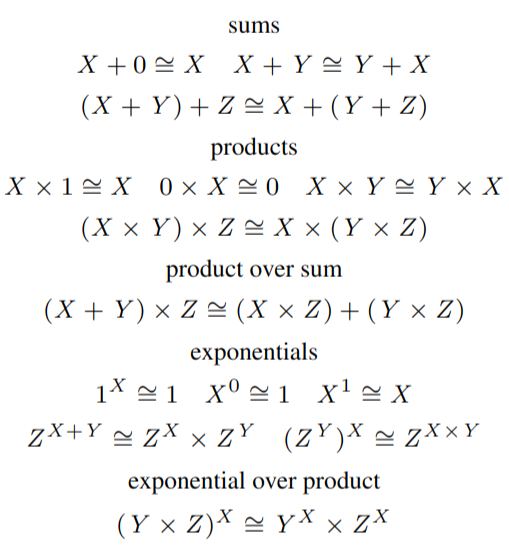
\includegraphics[width=1\textwidth]{figs/school-alg}
                \end{figure}
            \end{column}
        \end{columns}
    \end{frame}

    \begin{frame}[fragile]{Больше алгебры}
        \pause
        \begin{itemize}
            \item[\todo] Покажите, что $(a + b) + c \iso a + (b + c)$.
            \item[\todo] Покажите, что $c^{a + b} \iso c^a\times c^b$.
        \end{itemize}
        \pause\vspace{1em}
        \begin{minted}{haskell}
            -- ?$a \times a \iso a^2$?
            get :: (a, a) -> (Bool -> a)
            get (x, y) idx = if idx then x else y
            tabulate :: (Bool -> a) -> (a, a)
            tabulate f = (f True, f False)
        \end{minted}
    \end{frame}

    \begin{frame}[fragile]{Каноническое представление типа}
        \pause
        \[
            \sum_{i}\prod_{j} t_{ij}
        \]
    \end{frame}

    \sectionplan{Рекурсивные типы}

    \begin{frame}[fragile]{Рекурсивные типы}
        \begin{minted}{haskell}
            fac n = if n <= 1 then 1 else n * ?\framebox{fac}? (n - 1)
            data Nat = Zero | Suc ?\framebox{Nat}?
        \end{minted}
    \end{frame}

    \begin{frame}[fragile]{Список через неподвижную точку}
        \pause
        \begin{minted}{haskell}
            type Shape a r = Either () (a, r) -- ?$\lambda a~r\ldotp 1 + a\times r$?
            data FixList a = FixList (Shape a (FixList a))
            -- FixList a ?$\iso$? Shape a (FixList a) ?$\iso$? Shape a (Shape a (FixList a)) ?$\iso$? ...
        \end{minted}
        \vspace{1em}
        \begin{minted}{haskell}
            data [a] = [] | a : [a]
        \end{minted}
    \end{frame}

    \begin{frame}[fragile]{Свёртка}
        \pause
        \begin{center}
            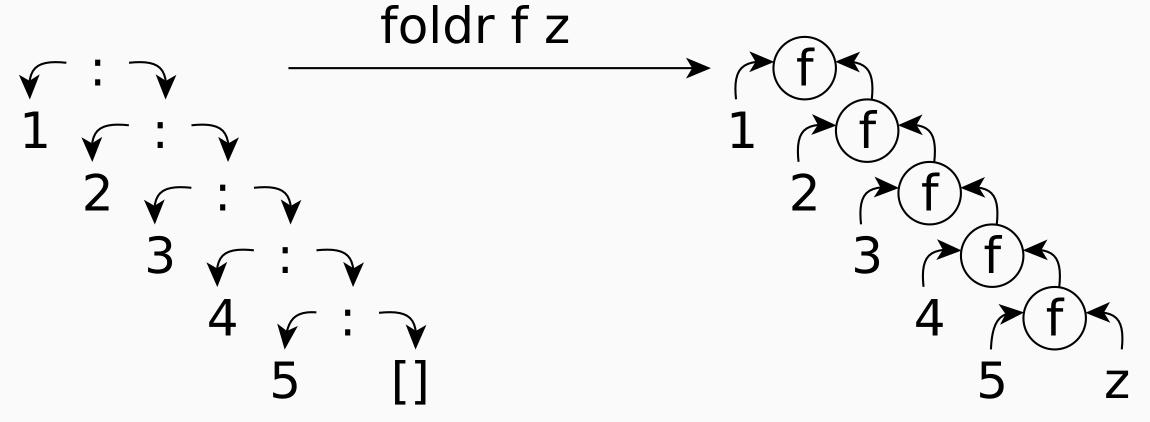
\includegraphics[width=0.7\textwidth]{figs/foldr}
        \end{center}
        \pause
        \begin{minted}{haskell}
            foldr :: (Either () (a, r) -> r) -> FixList a -> r
            foldr phi (FixList shape) = case shape of
              Left () -> phi (Left ())
              Right (x, xs) -> phi (Right (x, foldr phi xs))
            -- сравните с классическим определением
            foldr :: r -> (a -> r -> r) -> [a] -> r
        \end{minted}
    \end{frame}

    \begin{frame}[fragile]{Неподвижная точка функтора}
        \pause
        \begin{minted}{haskell}
            newtype Fix :: (Type -> Type) -> Type
            newtype Fix f = In { out :: f (Fix f) }

            data ListF a r = Nil | Cons a r
            type List a = Fix (ListF a)
        \end{minted}
        \pause\vspace{1em}
        \begin{minted}{haskell}
    to :: [a] -> List a
    to = \case
      [] -> In Nil
      x:xs -> In $ Cons x (to xs)

    from :: List a -> [a]
    from (In shape) = case shape of
      Nil -> []
      Cons x xs -> x : from xs
        \end{minted}
    \end{frame}

    \begin{frame}[fragile]{Функтор формы}
        \pause
        \begin{minted}{haskell}
            instance Functor (ListF a) where
              fmap :: (rec -> other) -> ListF a rec -> ListF a other
              fmap f = \case
                Nil -> Nil
                Cons x xs -> Cons x (f xs)
        \end{minted}
    \end{frame}

    \begin{frame}[fragile]{Катаморфизм}
        \pause
        \begin{minted}{haskell}
            cata :: Functor f => (f a -> a) -> Fix f -> a
            cata phi = phi . fmap (cata phi) . out
        \end{minted}
        \begin{figure}[h]
            \centering
            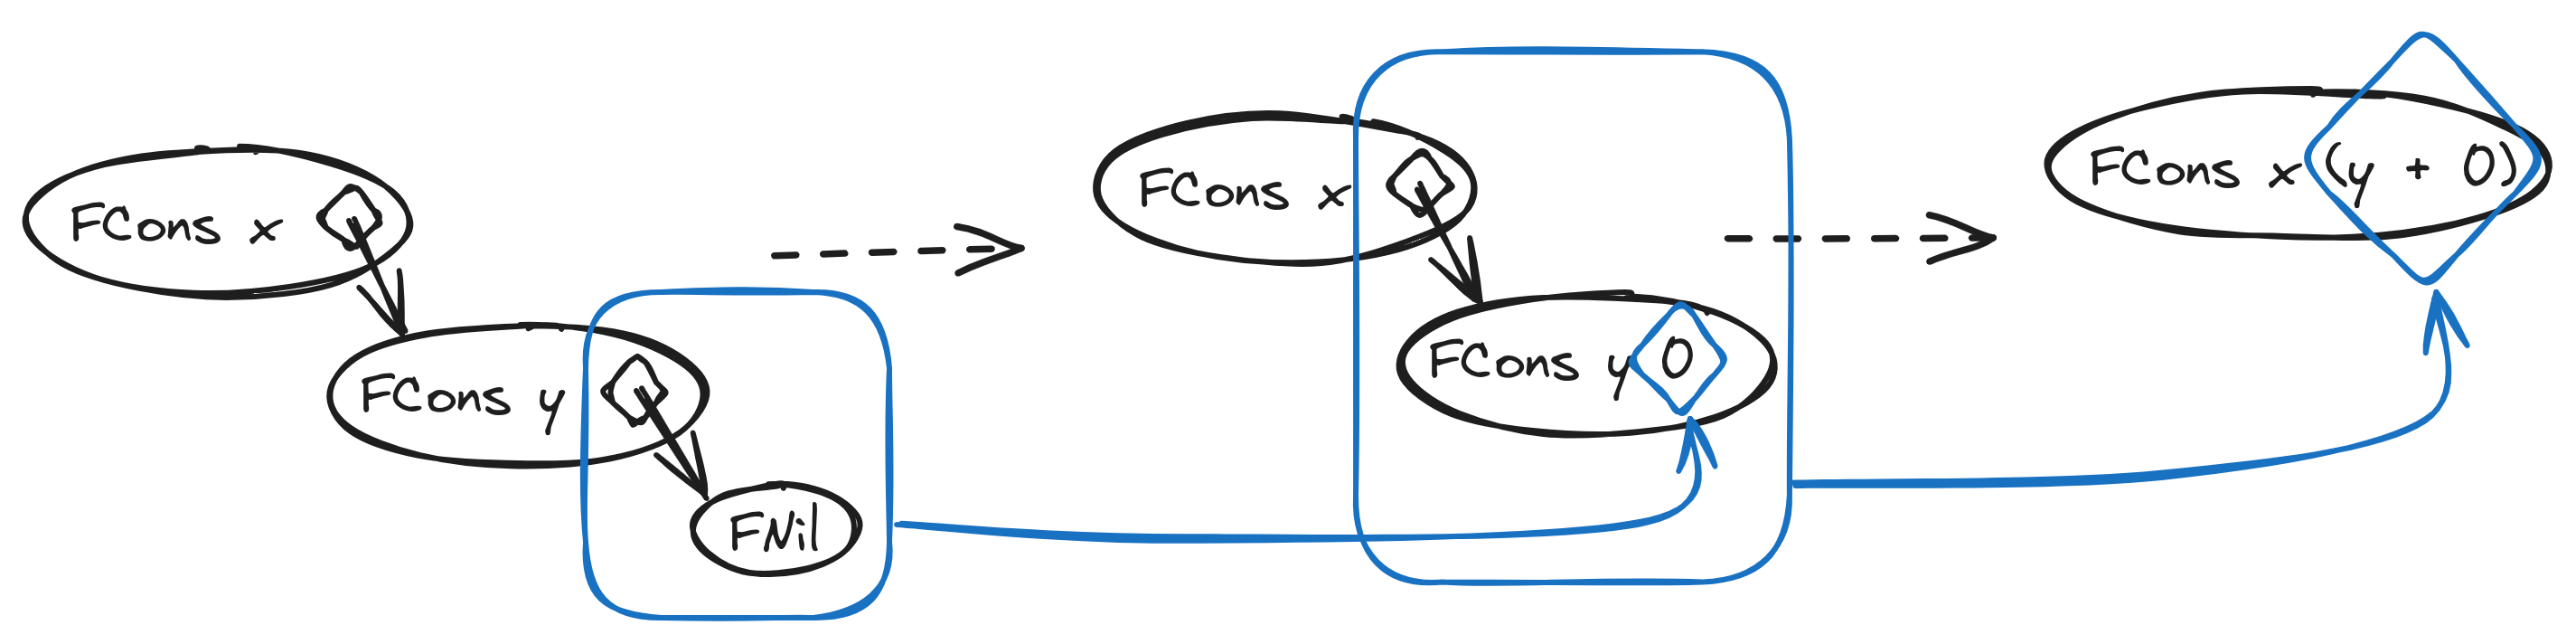
\includegraphics[width=0.8\textwidth]{figs/cataStep.excalidraw}
        \end{figure}
        \begin{minted}{haskell}
            sum :: List Int -> Int
            sum = cata \case
              Nil -> 0
              Cons x result -> x + result
        \end{minted}
    \end{frame}

    \begin{frame}[fragile]{Алгебры}
        \pause
        \begin{minted}{haskell}
            data MonoidSig carrier = Mempty | Mappend carrier carrier

            interpretSig :: MonoidSig Int -> Int
            interpretSig = \case Mempty -> 0; Mappend l r -> l + r
        \end{minted}
    \end{frame}

    \begin{frame}[fragile]{Анаморфизмы}
        \pause
        \begin{minted}{haskell}
            ana :: Functor f => (s -> f s) -> s -> Fix f
            ana psi = In . fmap (ana psi) . psi
            -- сравните с классическим определением развёртки списка
            unfoldr :: (s -> Maybe (a, s)) -> s -> [a]
        \end{minted}
    \end{frame}

    \begin{frame}[fragile]{Гилеморфизмы}
        \pause
        \begin{minted}{haskell}
    hylo :: Functor f => (a -> f a) -> (f b -> b) -> a -> b
    hylo psi phi = cata phi . ana psi
        \end{minted}
        \pause\vspace{1em}
        \begin{minted}{haskell}
    fac n = hylo
      (\n -> if n > 0 then Cons n (n - 1) else Nil)
      (\case Nil -> 1; Cons n acc -> n * acc)
        \end{minted}
    \end{frame}

    \sectionplan{Всё через свёртки}

    \begin{frame}[fragile]{Всё через свёртки}
        \pause
        \begin{minted}{haskell}
    to :: Functor f => Fix f -> (forall a . (f a -> a) -> a)
    to = flip cata

    from :: (forall a . (f a -> a) -> a) -> Fix f
    from g = g In
        \end{minted}
        \pause\vspace{1em}
        \begin{minted}{haskell}
    data ListF elem rec = Nil | Cons elem rec

    xs1 :: Fix (ListF Int)
    xs1 = In (Cons 1 (In (Cons 2 (In (Cons 3 (In Nil))))))

    xs2 :: (ListF Int a -> a) -> a
    xs2 = \alg -> alg (Cons 1 (alg (Cons 2 (alg (Cons 3 (alg Nil))))))

    ghci> xs2 @Int \case Nil -> 0; Cons x acc -> x + acc
    6
        \end{minted}
    \end{frame}

    \begin{frame}[fragile]{Список Чёрча}
        \pause
        \begin{align*}
            \text{\texttt{(ListF elem a -> a) -> a}}
            \iso a^{\displaystyle a^{\displaystyle 1 + elem\times a}}
            \iso a^{\displaystyle a\times a^{\displaystyle elem\times a}}
            \iso \left( a^{\displaystyle a} \right)^{\displaystyle \left(\left( a^{\displaystyle a}\right)^{\displaystyle elem}\right)} \\
            \iso \text{\texttt{a -> (elem -> a -> a) -> a}}
        \end{align*}
    \end{frame}

    \begin{frame}[fragile]{Дефорестация --- мотивация}
        \pause
        \begin{minted}{haskell}
    all p xs = and (map p xs)
    -- или fused версия
    all p [] = []
    all p (x:xs) = p x && all p xs
        \end{minted}
    \end{frame}

    \begin{frame}[fragile]{Дефорестация}
        \begin{figure}
            \centering
            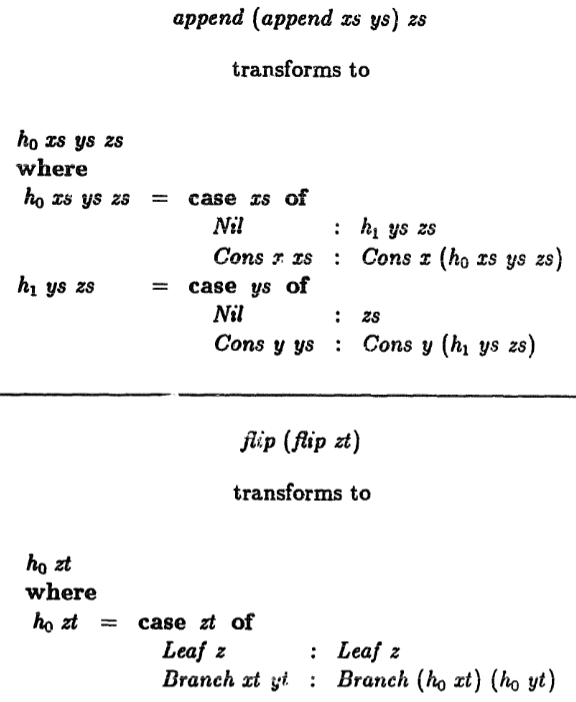
\includegraphics[width=0.6\textwidth]{figs/deforestation-examples}
        \end{figure}
    \end{frame}

    \begin{frame}[fragile]{List fusion}
        \pause
        \begin{minted}{haskell}
    {-# RULES
    "map/map" forall f g xs. map f (map g xs) = map (f . g) xs
      #-}
        \end{minted}
        \pause\vspace{1em}
        \begin{minted}{haskell}
    build :: (forall b . (a -> b -> b) -> b -> b) -> [a]
    build g = g (:) []
        \end{minted}
        \pause\vspace{1em}
        \begin{minted}{haskell}
    list123 :: [Int]
    list123 = build \s z -> s 1 (s 2 (s 3 z))

    map :: (a -> b) -> [a] -> [b]
    map f xs = build \s z -> foldr (\x acc -> s (f x) acc) z xs
        \end{minted}
        \pause\vspace{1em}
        \begin{minted}{haskell}
    foldr f ini (build g) ?$\equiv$? g f ini
        \end{minted}
    \end{frame}

    \begin{frame}[fragile]{Дефорестация вручную}
        \pause
        \begin{figure}
            \centering
            \begin{tabular}{p{0.5\textwidth} rl}
                \begin{minipage}[t]{0.5\textwidth}
                    \begin{minted}{cpp}
                std::variant<Msg1, Msg2>
                    deserialize(bytes bs) {
                    if (...) {
                        return std::variant{Msg1(...)};
                    else {
                        return std::variant{Msg2(...)};
                    }
                }
                    \end{minted}
                \end{minipage}
                &
                \begin{minipage}[t]{0.5\textwidth}
                    \begin{minted}{cpp}
                template<class Impl>
                auto deserialize(bytes bs) {
                    if (...) {
                        return Impl::processMsg1(...);
                    else {
                        return Impl::processMsg2(...);
                    }
                }
                    \end{minted}
                \end{minipage}
            \end{tabular}
        \end{figure}
    \end{frame}

    \begin{frame}[fragile]{Visitor pattern}
        \pause
        \begin{minted}{haskell}
    data Tree a = Leaf | Node a [Tree a]
    foldTree :: Tree a -> r -> (a -> [r] -> r) -> r
        \end{minted}
        \pause\vspace{1em}
        \begin{minted}{haskell}
    data Visitor a r = Visitor { onLeaf :: r, onNode :: a -> [r] -> r }
    visitTree :: Tree a -> Visitor a r -> r
        \end{minted}
        \pause\vspace{1em}
        \begin{minted}{haskell}
    data Tree a = Tree { visit :: forall r . Visitor a r -> r }

    leaf :: Tree a
    leaf = Tree { visit = \Visitor{onLeaf} -> onLeaf }

    node :: a -> [Tree a] -> Tree a
    node x ts = Tree { visit = \v@Visitor{onNode} -> onNode x (map (`visit` v) ts) }
        \end{minted}
    \end{frame}

    \begin{frame}[fragile]{Visitor pattern}
        \pause
        \begin{minted}{kotlin}
    interface Visitor<a, r> {
        fun onLeaf(): r
        fun onNode(x: a, subtrees: List<r>): r
    }

    interface Tree<a> {
        fun <r> visit(visitor: Visitor<a, r>): r
    }
    class Leaf : Tree<Nothing> {
        override fun <r> visit(visitor: Visitor<Nothing, r>): r = visitor.onLeaf()
    }
    class Node<a>(val value: a, val subtrees: List<Tree<a>>) : Tree<a> {
        override fun <r> visit(visitor: Visitor<a, r>): r =
            visitor.onNode(value, subtrees.map { it -> it.visit(visitor) })
    }
        \end{minted}
    \end{frame}

    \sectionplan{Всё через развёртку}

    \begin{frame}[fragile]{Всё через развёртку}
        \pause
        \begin{minted}{haskell}
    ana :: Functor f => forall s . (s -> f s) -> s -> Fix f
    ana psi = In . fmap (ana psi) . psi
        \end{minted}
        \pause\vspace{1em}
        \begin{minted}{haskell}
    ana :: Functor f => (exists s . (s, s -> f s)) -> Fix f
        \end{minted}
        \pause\vspace{1em}
        \begin{minted}{haskell}
    data Box f where
      --     exists s. (s,    s -> f s)
      Box :: forall s . s -> (s -> f s) -> Box

    ana' :: Functor f => Box f -> Fix f
    ana' (Box currSeed psi) =
      In $ (\nextSeed -> ana' (Box nextSeed psi)) <$> psi currSeed
        \end{minted}
    \end{frame}

    \begin{frame}[fragile]{Изоморфизм}
        \pause
        \begin{minted}{haskell}
            to :: Fix f -> Box f
            to x = Box x out

            from :: Functor f => Box f -> Fix f
            from = ana'
        \end{minted}
        \pause\vspace{1em}
        \begin{minted}{haskell}
    nats :: Box (ListF Int)
    nats = Box 0 \curr -> Cons curr (curr + 1)
        \end{minted}
    \end{frame}

    \begin{frame}[fragile]{Stream fusion}
        \pause
        \begin{minted}{haskell}
    data ListF a r = Nil | Cons a r
    type MyStream a = Box (ListF a) -- ?$\exists$?s . (s -> ListF a s, s)
    -- ?$\iso$?
    data Step a s = Done | Yield a s
    data Stream a where
      Stream :: forall s . (s -> Step a s) -> s -> Stream a

    stream :: [a] -> Stream a
    stream xs = Stream (\case [] -> Done; x:xs -> Yield x xs) xs

    unstream :: Stream a -> [a]
    unstream (Stream next s) = case next s of
      Done -> []
      Cons a s' -> a : unstream next s'
        \end{minted}
    \end{frame}

    \begin{frame}[fragile]{Пример map}
        \begin{minted}{haskell}
    mapS :: (a -> b) -> Stream a -> Stream b
    mapS f (Stream next s) = Stream next' s
      where
        next' s = case next s of
          Done -> Done
          Yield x s' -> Yield (f x) s'
        \end{minted}
    \end{frame}

    \begin{frame}[fragile]{Общий пайплайн}
        \pause
        \begin{enumerate}
            \item Мы пишем все функции работы со списками через стримы:
            \begin{minted}{haskell}
        map :: (a -> b) -> [a] -> [b]
        map f = unstream . map f . stream
            \end{minted}
            \item С помощью RULES задаём правило переписывания stream/unstream, двойственное foldr/build: \texttt{stream . unstream = id}.
            \item Далее справляются обычные компиляторные оптимизации.
        \end{enumerate}
    \end{frame}

    \begin{frame}[fragile]{Фильтрация стримов}
        \begin{minted}{haskell}
    data Step a s = Done | Skip s | Yield a s

    filterS :: (a -> Bool) -> Stream a -> Stream a
    filterS p (Stream next s) = Stream next' s
      where
        next' s = case next s of
          Done -> Done
          Skip s' -> Skip s'
          Yield a s' -> if p a then Yield a s' else Skip s'
        \end{minted}
    \end{frame}

    \sectionplan{Вездесущий дуализм}

    \begin{frame}[fragile]{Push vs pull streaming}
        \pause
        \begin{minted}{kotlin}
    events.observe(object : Observer<Event> {
        override fun onComplete() { .. }
        override fun onNext(elem: Event) { .. }
    })
        \end{minted}
    \end{frame}

    \begin{frame}[fragile]{Data vs codata}
        \pause
        \begin{minted}{haskell}
    data ListF a r = Nil | Cons a r
        \end{minted}
        \pause\vspace{1em}
        \begin{minted}{haskell}
            data List a where
              List :: ListF a (List a) -> List a

            fold :: (ListF a r -> r) -> List a -> r
            fold alg xs = case xs of
              Fix Nil -> alg Nil
              Fix (Cons y ys) -> alg (Cons y (fold alg ys))
        \end{minted}
        \pause\vspace{1em}
        \begin{minted}{haskell}
    codata CoList a where
      force :: CoList a -> ListF a (CoList a)

    unfold :: (s -> ListF a s) -> s -> CoList a
    force (unfold coalg s) = case coalg s of
      Nil -> Nil
      Cons x s' -> Cons x (unfold coalg s')
        \end{minted}
    \end{frame}

    \begin{frame}[fragile]{OOP}
        \pause
        \begin{minted}[escapeinside=**]{kotlin}
    class List<a>(val layer: Pair<a, List<a>>?)

    fun <a, r> fold(alg: (Pair<a, r>?) -> r, xs: List<a>): r =
        if (xs.layer == null) alg(null)
        else alg(Pair(xs.layer.first, fold(alg, xs.list.second)))

    interface CoList<a> { fun force(): Pair<a, CoList<a>>? }

    fun <a, s> unfold(coalg: (s) -> Pair<a, s>?, ini: s): CoList<a> =
        object : CoList<a> {
            override fun force(): Pair<a, CoList<a>>? {
                val layer = coalg(ini)
                return if (layer == null) null else
                    Pair(layer.first, unfold(coalg, layer.second))
            }
        }
        \end{minted}
    \end{frame}

\end{document}
